Results for \detdeta using EMCal, HCal and Full Calorimeter data are presented as a function of $\eta$ for centrality bins within the range $0$--$70$\% in Figure~\ref{fig:detdeta_full_cent_range}. 
The \detdeta values have a strong dependence on centrality, varying by more than a factor of 10 between the most peripheral and most central events considered here. 
The measurements using each of the three methods (EMCal-only, HCal-only, and the full calorimeter system) shown in Figure~\ref{fig:detdeta_full_cent_range} have compatible results within uncertainties across all centrality bins and $\eta$ values.
Additionally, no significant dependence on $\eta$ is observed within the range $\left|\eta\right| < 1.1$.
The measurements at the same absolute value of $\eta$ are generally consistent across all methods and centralities. 
Small deviations, up to a few percent, are observed at forward-$\left|\eta\right|$ in the most central intervals and are accounted for within the total estimated uncertainties.
The symmetry of the measurements with respect to $\eta$ is highlighted in Figure~\ref{fig:flipped_detdeta_full_cent_range}, where the EMCal, HCal and Full Calorimeter results are overlaid by these measurements flipped across $\eta$ = 0.

\begin{figure}[t]
    \centering
    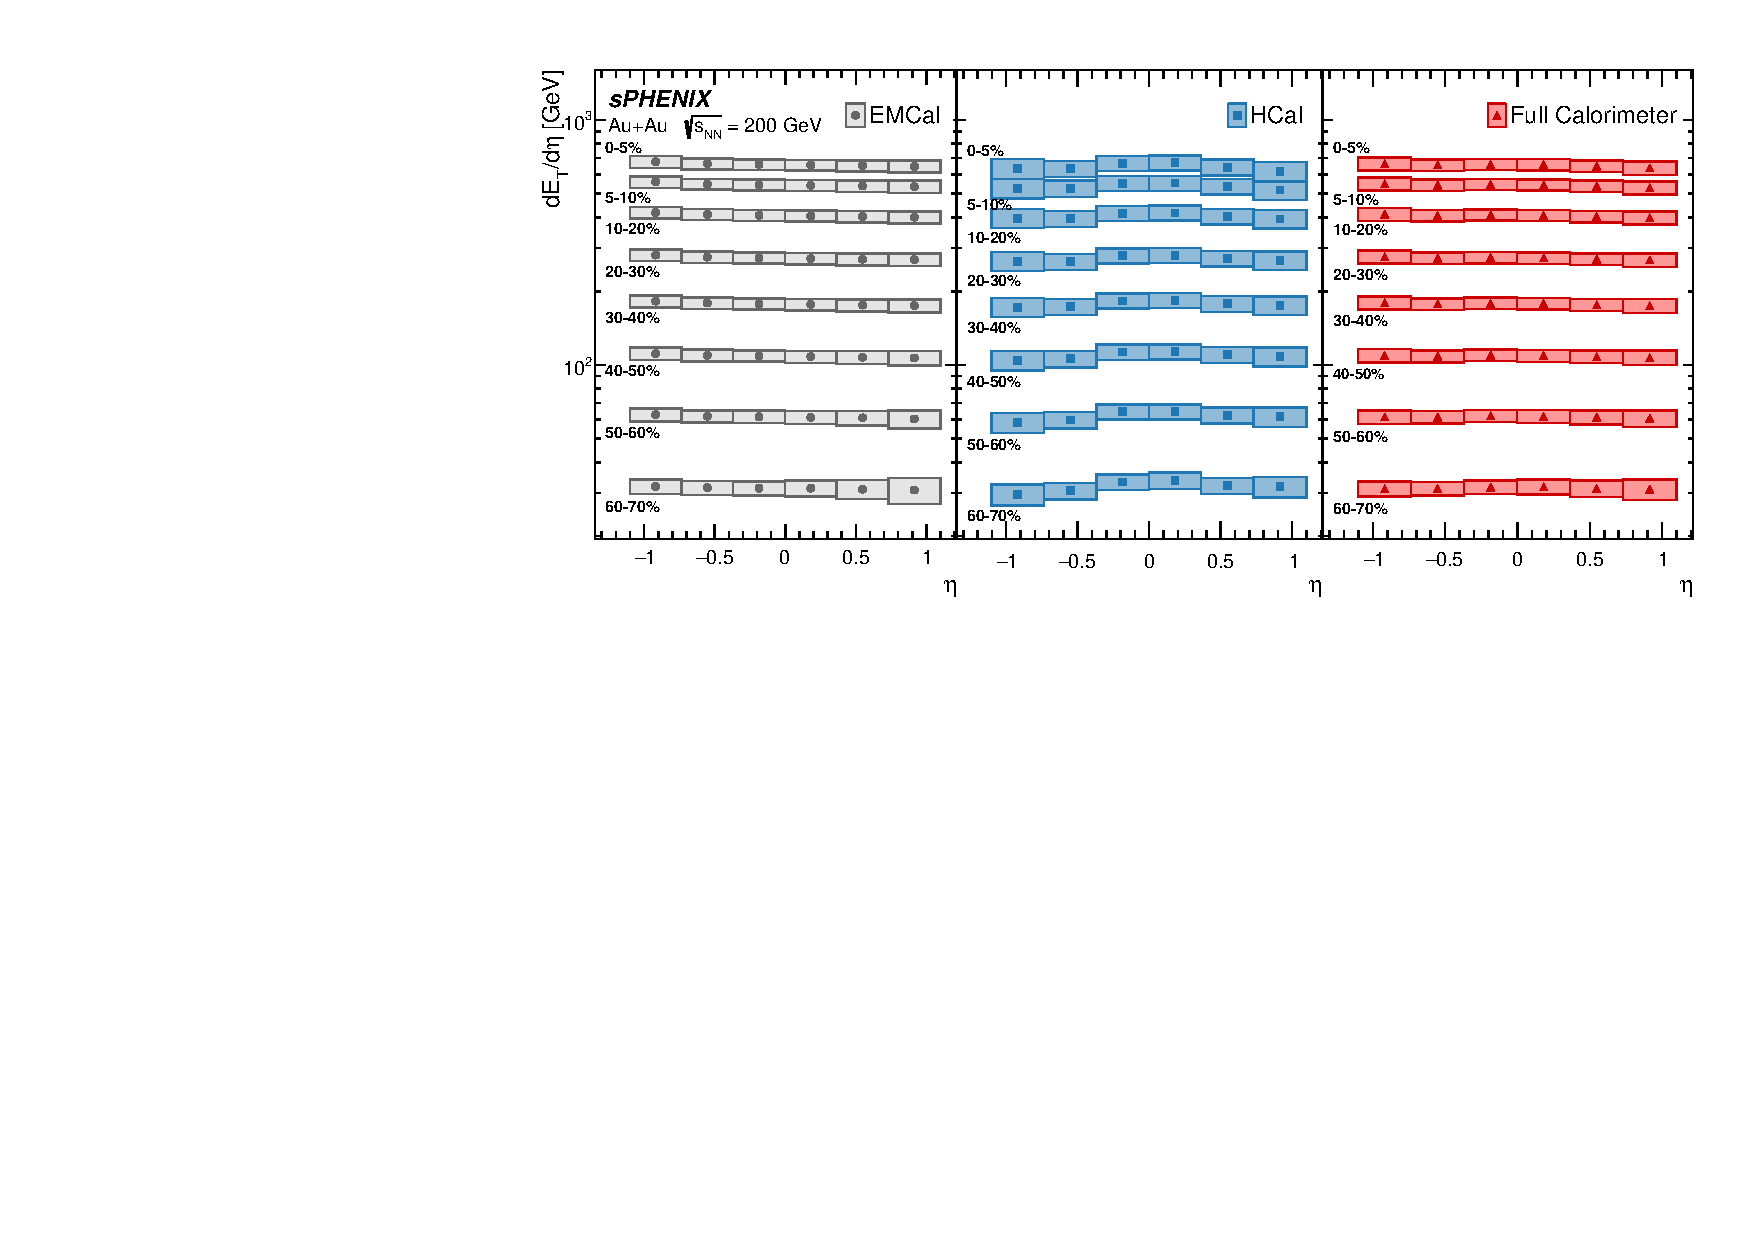
\includegraphics[width=\linewidth]{figures/chapter4/emcal_hcal_calo_detdeta_separate_final_prc_edit.pdf}
    \caption{Summary of \detdeta measurements in Au+Au collisions at $\sqrt{s_\mathrm{_{NN}}} = 200$~GeV over the pseudorapidity range $\left|\eta\right| < 1.1$. Different data series correspond to centrality selections within the range $0$--$70$\% (labeled). The different panels show the results determined using the EMCal-only (left), HCal-only (center), and the full calorimeter system (right). The vertical size of the boxes around each point indicate the total systematic uncertainty, while the horizontal size indicates the $\eta$ bin width.}
    \label{fig:detdeta_full_cent_range}
\end{figure}

\begin{figure}
    \centering
    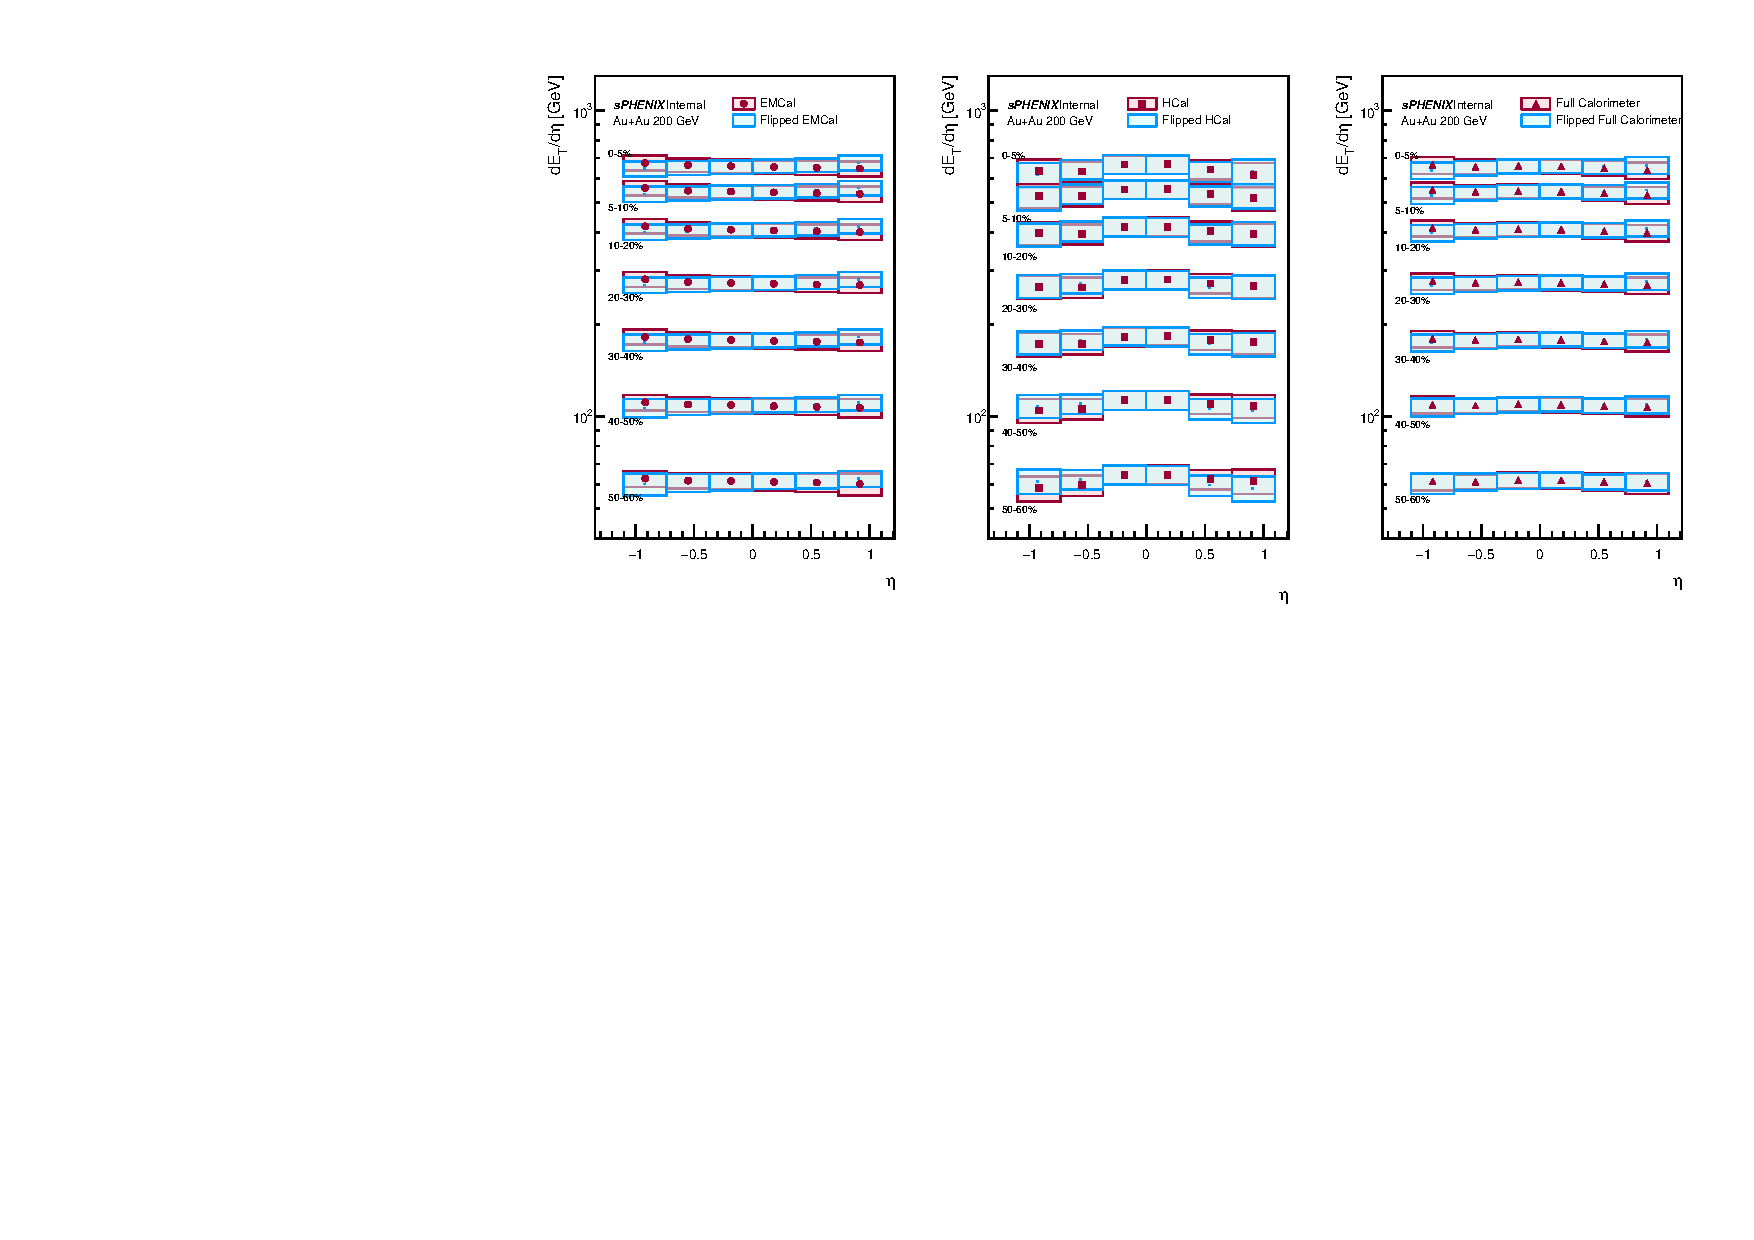
\includegraphics[width=\linewidth]{detdeta/Figures/dETdeta_measurements/flipped_emcal_hcal_full_calo_all_cent_log_separate_1.pdf}
    \caption{Results of \detdeta over measurement range $-1.1<\eta<1.1$ for EMCal (left), HCal (middle) and Full Calorimeter (right) data shown in red. Measurements over centrality range from 0-5\% to 50-60\% are presented for all calorimeter configuration measurements. \detdeta measurements flipped about $\eta$ = 0 overlaid in blue to highlight symmetry in the measurements about $\eta$ = 0.}
    \label{fig:flipped_detdeta_full_cent_range}
\end{figure}

Results using all calorimeter configurations (EMCal-only, HCal-only, IHCal-only, OHCal-only and Full Calorimeter) of the average $\detdeta$ per participant pair, $\Npart$/2, as a function of $\Npart$, are shown in Figure~\ref{fig:dETdeta_npart_all_calo_layers}. 
The $\langle \detdeta\rangle/(0.5 \Npart)$ values show a gradual increase for more central collisions (i.e. higher \Npart) irrespective of various calorimeter configurations used and good agreement over the full \Npart range is seen for the EMCal, HCal, Full Calorimeter and OHCal-only measurements;
the IHCal-only measurement is consistently higher than the other measurements, but sees only 4\% of the collision energy due to the small interaction length of the IHCal making it unable to capture the full dynamics of the total collision energy with the same accuracy as the other two calorimeter subsystems which see a much larger fraction of the collision energy. 

\begin{figure}
    \centering
    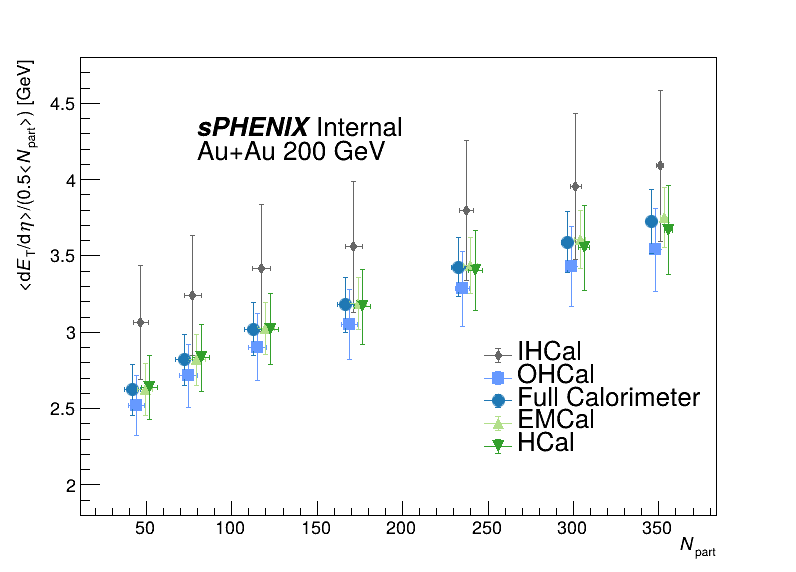
\includegraphics[height=3.6in]{detdeta/Figures/dETdeta_measurements/dETdeta_Npart_vs_Npart_all_calo_layers.png}
    \caption{Mean \detdeta over 0.5\Npart as a function of \Npart for EMCal, HCal, IHCal-only, OHCal-only and full calorimeter measurement. Uncertainty bands on measurements correspond to the quadrature sum of the errors on \detdeta measurement and the uncertainties on the \Npart calculation.}
    \label{fig:dETdeta_npart_all_calo_layers}
\end{figure}

In Figure~\ref{fig:emcal_hcal_comp}, the EMCal-only and HCal-only \detdeta measurements in the most central 0--5\% Au+Au events are overlaid to highlight their agreement. 
The EMCal and HCal have independent calibration sequences and are sensitive to the energy from different particles of the collision. 
Therefore, this good agreement between the EMCal-only and HCal-only measurements helps validate the sPHENIX calorimeter reconstruction, calibrations and simulation.
Figure~\ref{fig:emcal_hcal_comp} also includes comparisons to previous STAR~\cite{STAR_detdeta} and PHENIX~\cite{PHENIX_detdeta} results for the most central 0--5\% Au+Au events.
For comparison, the STAR results measured from $0 < \eta < 1$ are symmetrized over range $|\eta| < 1$. Both the sPHENIX EMCal-only and HCal-only measurements are compatible with the previous measurements at RHIC performed using only electromagnetic calorimetry or a combination of tracking detectors and an electromagnetic calorimeter, while providing additional granularity in $\eta$.
For this centrality range, the total uncertainties are comparable between the sPHENIX, PHENIX, and STAR measurements. The uncertainties for the sPHENIX EMCal-only results are similar in magnitude to that for the previous PHENIX results, which also used only an EM calorimeter for the \detdeta measurement.

\begin{figure}[h]
    \centering
    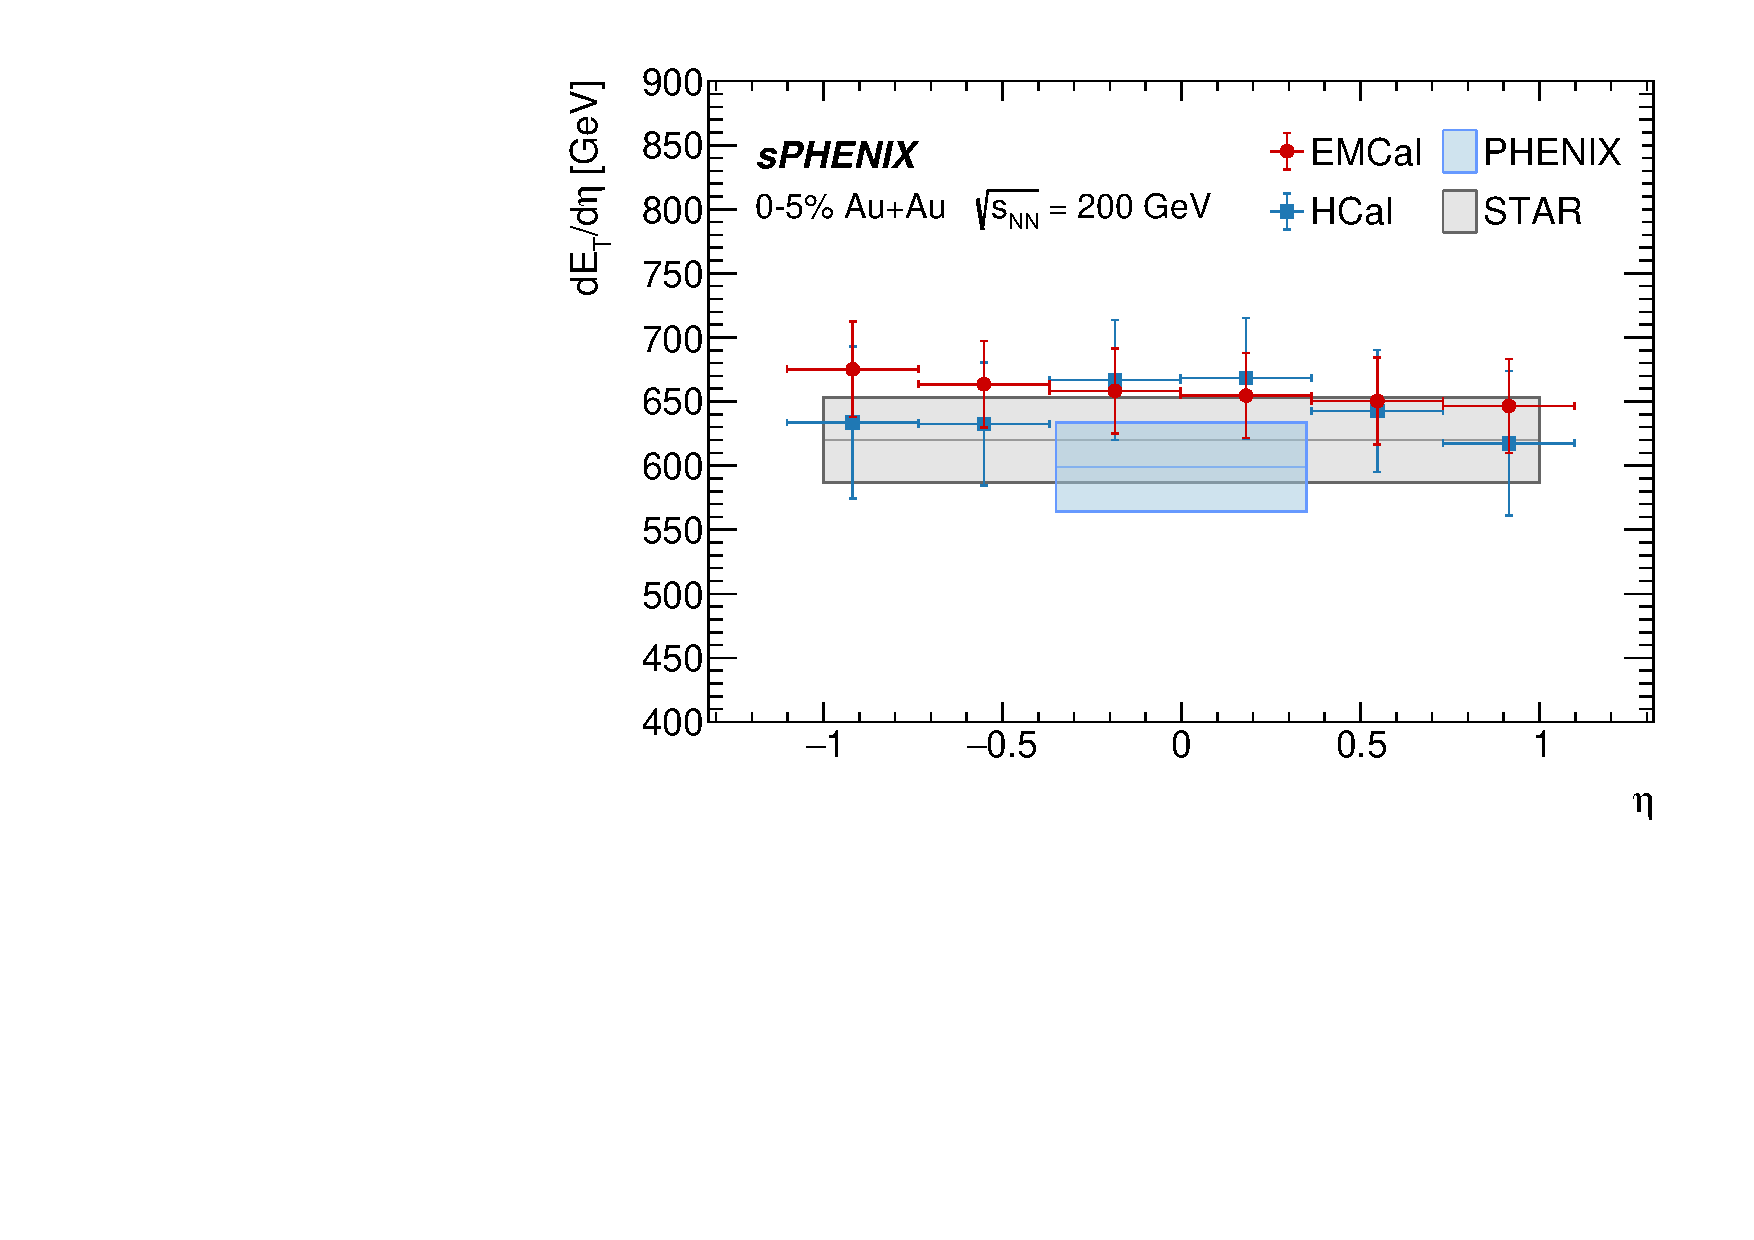
\includegraphics[height=3.6in]{figures/chapter4/emcal_hcal_star_phenix_detdeta_0_5_final.pdf}
    \caption{Measurement of \detdeta in 0--5\% central \auau{} events using only EMCal (red points) and only HCal (blue points), as a function of $\eta$ over the range $\left|\eta\right| < 1.1$. The vertical error bars show the total systematic uncertainty. The measurements from PHENIX~\cite{PHENIX_detdeta} (blue box) and STAR~\cite{STAR_detdeta} (gray box) in this centrality interval are shown for comparison, with the vertical and horizontal size of the box indicating the total uncertainty and the measurement range in $\eta$, respectively.}
    \label{fig:emcal_hcal_comp}
\end{figure}

Figure~\ref{fig:detdeta_vs_npart} shows the average \detdeta, normalized by participant pair as a function of \Npart, measured using the full sPHENIX calorimeter system.
The values of $\langle \detdeta\rangle/(0.5 \Npart)$ gradually increase across the measurement's \Npart range, from approximately 2.5 GeV to 3.5 GeV per participant pair over the reported \Npart range.
The sPHENIX full calorimeter results are compared to previous results from PHENIX \cite{PHENIX_detdeta} and STAR \cite{STAR_detdeta}. 
The sPHENIX measurement is in agreement with the previous measurements from PHENIX and STAR and features improved precision in peripheral events.
Figure~\ref{fig:detdeta_vs_npart} also shows comparisons to the generator-level $\langle \detdeta\rangle/(0.5 \Npart)$ from \hijing, \epos and \ampt (each without the applied reweighting used for the analysis correction factors);
\ampt best describes the magnitude and trend with \Npart of the \detdeta across the full \Npart range measured by sPHENIX.

\begin{figure}[h]
    \centering
    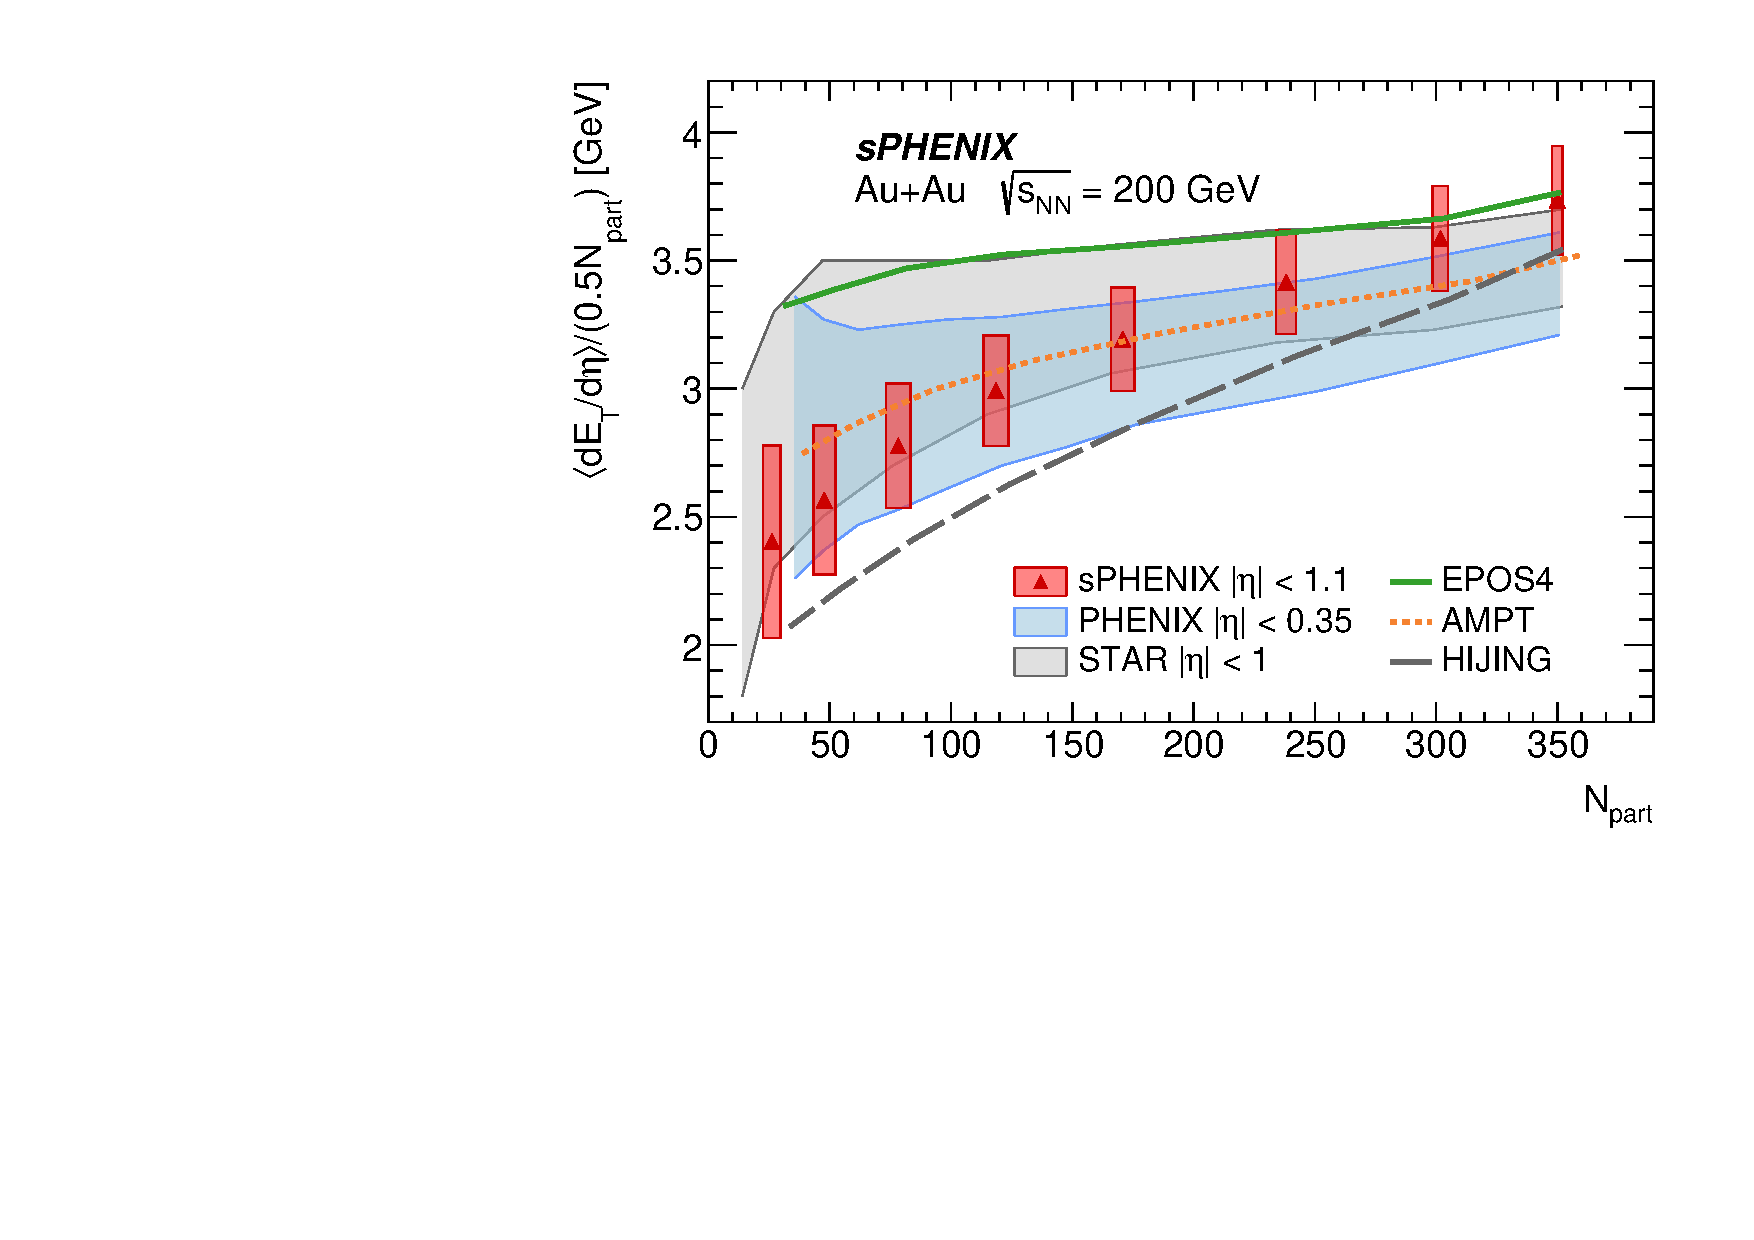
\includegraphics[height=3.6in]{figures/chapter4/dETdeta_Npart_vs_Npart_detector_comp_rw_epos_wstarphenixline_final_prc_edit.pdf}
    \caption{Measured \detdeta normalized by the estimated number of participant pairs ($0.5$\Npart), as a function of \Npart, using the full calorimeter system (red triangles). The vertical size of the boxes indicates the total uncertainty, which includes the uncertainty in \Npart. Measurements by PHENIX~\cite{PHENIX_detdeta} (blue band) and STAR~\cite{STAR_detdeta} (gray band) are shown for comparison, with the vertical size of the band indicating the uncertainty range. MC event generator predictions are shown for \epos (solid green line), \ampt (dotted orange line), and \hijing (dashed black line).}
    \label{fig:detdeta_vs_npart}
\end{figure}